%!TEX root = SISC_elastic_3d.tex
\subsection{Semi-discretization of the elastic wave equation}\label{semi_discrete_form}

\begin{figure}[htbp]
	\centering
	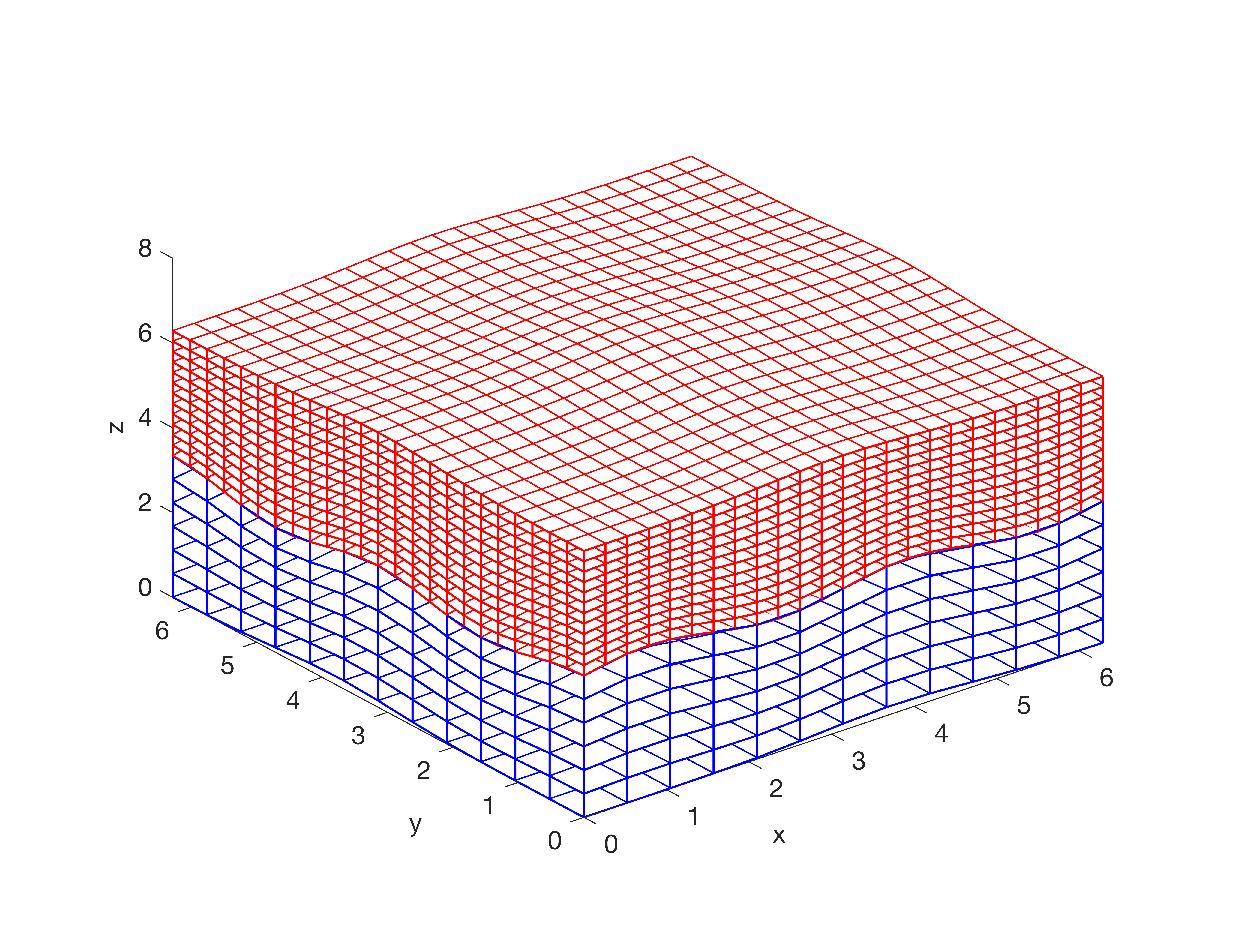
\includegraphics[width=0.6\textwidth,trim={0.4cm 0.7cm 0.8cm 1.4cm}, clip]{physical_discretization.eps}
	\caption{The sketch for the curvilinear mesh of the physical domain $\Omega$. The blue region is the spatial discretization of coarse subdomain $\Omega^c$ and the red region is the spatial discretization of the fine domain $\Omega^f$. Note that $x,y,z$ in the graph correspond to $x^{(1)}, x^{(2)}, x^{(3)}$ respectively. 
	 }\label{physical_discretization}
\end{figure}

In this section, we discretize the elastic wave equations (\ref{elastic_curvi}) and  (\ref{elastic_curvi_f}) with mesh refinement interface $\Gamma$. We assume the ratio of mesh sizes in the reference domains is $1:2$, that is the mesh sizes satisfy
\[h_1(n_1^h-1) = 1, \ \ \ h_2(n_2^h-1) = 1, \ \ \ h_3(n_3^h-1) = 1,\]
and
\[2h_1(n_1^{2h}-1) = 1, \ \ \ 2h_2(n_2^{2h}-1) = 1, \ \ \ 2h_3(n_3^{2h}-1) = 1,\]
respectively. Other ratios can be treated analogously. Figure \ref{physical_discretization} gives an illustration of the discretization of a physical domain. This is an ideal mesh if the wave speed in $\Omega^f$ is half of the wave speed in $\Omega^c$.

In seismic wave simulation, far-field boundary conditions are often imposed in the $x^{(1)}$ and $x^{(2)}$ directions. Here, our focus is on the numerical treatment of the interface conditions (\ref{interface_cond}). We assume periodic boundary conditions in $x^{(1)}$ and $x^{(2)}$, and ignore the boundaries in $x^{(3)}$. In Figure \ref{section_discretization}, we fix $x^{(2)} = 0$ and present the $x^{(1)}$-$x^{(3)}$ section of the domain $\Omega$ in both curvilinear space and parameter space.
\begin{figure}[htbp]
	\centering
	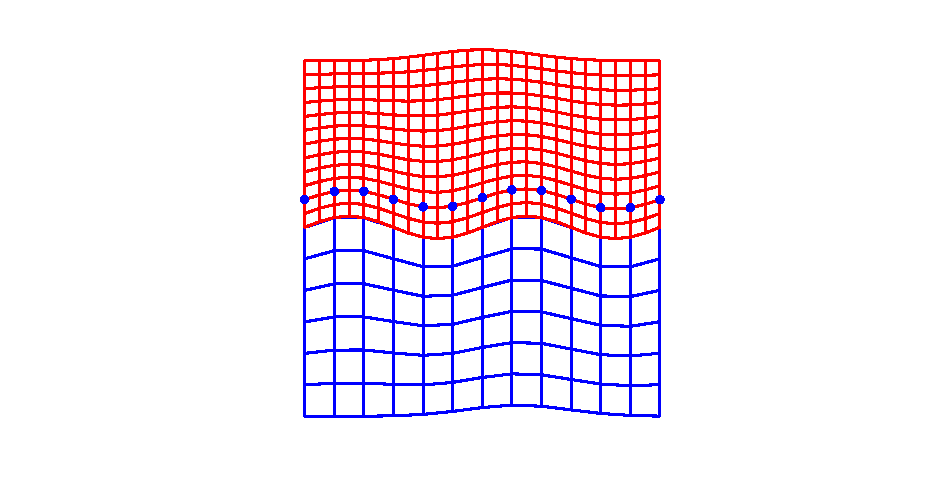
\includegraphics[width=0.45\textwidth,trim={1.0cm 2.0cm 1.0cm 1.8cm}, clip]{physical_section_discretization.eps}
	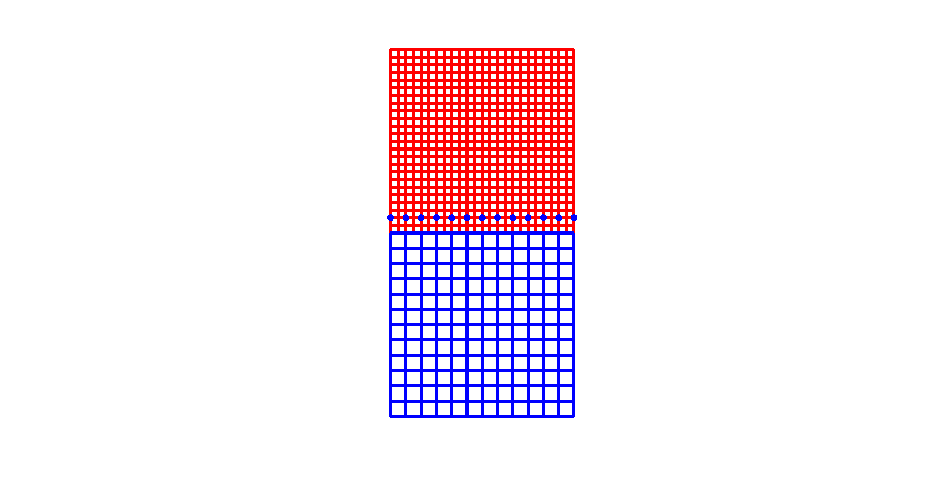
\includegraphics[width=0.45\textwidth,trim={1.0cm 2.0cm 1cm 1.8cm}, clip]{parameter_section_discretization.eps}
	\caption{The sketch of spatial discretization of $x^{(1)}$-$x^{(3)}$ section with $x^{(2)} = 0$. From the left to the right are for physical domain and parameter space, respectively. The blue dots are the ghost points for the coarse domain $\Omega^c$.}\label{section_discretization}
\end{figure}
 To condense notations, we introduce the multi-index notations
\[{\bf i} = (i,j,k),\ \ {\bf r}_{\bf i} = (r^{(1)}_i,r^{(2)}_j,r^{(3)}_k),\ \ {\bf x}_{\bf i} = (x^{(1)}_i,x^{(2)}_j,x^{(3)}_k),\]
then group different sets of grids as
\begin{equation*}
\begin{aligned}
	I_{\Omega^c} &= \{i = 1,2,\cdots,n_1^{2h}, j = 1,2,\cdots,n_2^{2h}, k = 1,2,\cdots,n_3^{2h}\},\\
	I_{\Gamma^c} & = \{i = 1,2,\cdots,n_1^{2h}, j = 1,2,\cdots,n_2^{2h}, k = n_3^{2h}\},\\
	I_{\Gamma^f} & = \{i = 1,2,\cdots,n_1^{h}, j = 1,2,\cdots,n_2^{h}, k = 1\},\\
	I_{\Omega^f} &= \{i = 1,2,\cdots,n_1^h, j = 1,2,\cdots,n_2^h, k = 1,2,\cdots,n_3^h\}.
\end{aligned}	
\end{equation*}
The physical coordinates of the coarse grid points and fine grid points follow from the mappings ${\bf x}_{\bf i} = {\bf X}^c({\bf r}_{\bf i})$ and ${\bf x}_{\bf i} = {\bf X}^f({\bf r}_{\bf i})$, respectively. We denote a grid function by
\[{\bf u}_{\bf i} = {\bf u}_{i,j,k} = {\bf u}({\bf x}_{\bf i}),\]
where ${\bf u}$ can be either a scalar or vector. Then we approximate the elastic wave equation (\ref{elastic_curvi}) in $\Omega^c$ by
\begin{equation}\label{elastic_semi_c}
{\rho}_{\bf i}^{c}\frac{d^2{{\bf C}_{\bf i}}}{dt^2} = \frac{1}{J^c_{\bf i}}\wt{\mathcal{L}}^{2h} {{\bf C}}_{\bf i},\quad {\bf i}\in I_{\Omega^c},\quad t>0,
\end{equation}
where the discrete spatial operator is
\begin{equation}\label{L_operator}
\wt{\mathcal{L}}^{2h} {{\bf C}} = \left(\sum_{l=1}^2{Q}_l^{2h}({N}_{ll}^{2h}){\bf C}+\wt{{G}}_3^{2h}({N}_{33}^{2h}){{\bf C}}+\sum_{l=1}^3\sum_{m=1,m\neq l}^3{D}_l^{2h}({N}_{lm}^{2h}{D}_m^{2h}{\bf C})\right).
\end{equation}
Here, the components of the vector ${\bf C}$ are ${\bf C} = (C^{(1)}, C^{(2)}, C^{(3)})^T$. For the fisrt term in (\ref{L_operator}), we have
\begin{align*}
{Q}_l^{2h}({N}_{ll}^{2h}){\bf C} := \left(\begin{array}{c}
({Q}_l^{2h}({N}_{ll}^{2h}){\bf C})_1 \\
({Q}_l^{2h}({N}_{ll}^{2h}){\bf C})_2 \\
({Q}_l^{2h}({N}_{ll}^{2h}){\bf C})_3 
\end{array}\right), \quad ({Q}_l^{2h}({N}_{ll}^{2h}){\bf C})_p = \sum_{q = 1}^{3} Q_l^{2h}(N_{ll}^{2h}(p,q)) {C}^{(q)},\quad p = 1,2,3,
\end{align*}
where we have used a matlab notation $N_{ll}^{2h}(p,q)$ to represent the $p'$th row and $q'$th column of the matrix $N_{ll}^{2h}$; $Q_l^{2h}(N_{ll}^{2h}(p,q)){ C}^{(q)}$ is the central difference operator in direction $r^{(l)}$ for spatial second derivative with variable coefficient. For the second term in (\ref{L_operator}), we have
\begin{align*}
\wt{{G}}_3^{2h}({N}_{33}^{2h}){\bf C} := \left(\begin{array}{c}
(\wt{{G}}_3^{2h}({N}_{33}^{2h}){\bf C})_1 \\
(\wt{{G}}_3^{2h}({N}_{33}^{2h}){\bf C})_2 \\
(\wt{{G}}_3^{2h}({N}_{33}^{2h}){\bf C})_3 
\end{array}\right), \quad (\wt{{G}}_3^{2h}({N}_{33}^{2h}){\bf C})_p = \sum_{q = 1}^{3} \wt{G}_3^{2h}(N_{33}^{2h}(p,q)) {C}^{(q)},\quad p = 1,2,3,
\end{align*}
where $\wt{G}_3^{2h}(N_{33}^{2h}(p,q)) { C}^{(j)}$ is the scalar difference operator which is defined in (\ref{sbp_2nd_1}) for direction $r^{(3)}$. For the third term in (\ref{L_operator}), we have
\begin{align*}
{D}_l^{2h}({N}_{lm}^{2h}{D}_m^{2h}{\bf C}) := \left(\begin{array}{c}
(D^{2h}_l(N^{2h}_{lm}D_m^{2h}{\bf C}))_1 \\
(D^{2h}_l(N^{2h}_{lm}D_m^{2h}{\bf C}))_2 \\
(D^{2h}_l(N^{2h}_{lm}D_m^{2h}{\bf C}))_3 
\end{array}\right), \quad (D^{2h}_l(N^{2h}_{lm}D_m^{2h}{\bf C}))_p = \sum_{q = 1}^{3} D^{2h}_l(N^{2h}_{lm}(p,q)D_m^{2h}{C}^{(q)}),
\end{align*}
$p = 1,2,3$. Here, $D_m^{2h}C^{(q)}, m = 1,2$ are central difference operator in direction $r^{(m)}$ for the spatial first derivative, and $D_3^{2h}C^{(q)}$ is the scalar difference operator defined in (\ref{first_sbp}) for direction $r^{(3)}$.

Next, we approximate the elastic wave equation (\ref{elastic_curvi_f}) for the fine grids. We first consider all fine grid points which are not located at the interface $\Gamma$, and have the semi-discretization
\begin{equation}\label{elastic_semi_f}
{\rho}_{\bf i}^{f}\frac{d^2{{\bf F}_{\bf i}}}{dt^2} = \frac{1}{J^f_{\bf i}}{\mathcal{L}}^{h} {{\bf F}}_{\bf i},\quad {\bf i}\in I_{\Omega^f}\backslash I_{{\Gamma^f}},\quad t>0,
\end{equation}
where the discrete spatial operator is
\begin{equation}\label{Lf_operator}
{\mathcal{L}}^{h} {{\bf F}} = \left(\sum_{l=1}^2{Q}_l^{h}({N}_{ll}^h){\bf F}+{G}_3^{h}({N}_{33}^h){\bf F}+\sum_{l=1}^3\sum_{m=1,m\neq l}^3{D}_l^{h}({N}_{lm}^{h}{D}_m^{h}{\bf F})\right),
\end{equation}
where the components of the vector ${\bf F}$ are ${\bf F} = (F^{(1)}, F^{(2)}, F^{(3)})$. In addition, ${Q}_l^{h}({N}_{ll}^h){\bf F}, l = 1,2$ and ${D}_l^{h}({N}_{lm}^{h}{D}_m^{h}{\bf F})$ are defined similar as those in (\ref{L_operator}), but with the grids in $I_{\Omega^f}\backslash I_{{\Gamma^f}}$. And
\begin{align*}
{{G}}_3^{h}({N}_{33}^{h}){\bf F} := \left(\begin{array}{c}
({{G}}_3^{h}({N}_{33}^{h}){\bf F})_1 \\
({{G}}_3^{h}({N}_{33}^{h}){\bf F})_2 \\
({{G}}_3^{h}({N}_{33}^{h}){\bf F})_3 
\end{array}\right), \quad ({{G}}_3^{h}({N}_{33}^{h}){\bf F})_p = \sum_{q = 1}^{3} {G}_3^{h}(N_{33}^{h}(p,q)) {F}^{(q)},\quad p = 1,2,3.
\end{align*}
Here, ${G}_3^{h}(N_{33}^{h}(p,q)) {F}^{(q)}$ is a scalar difference operator defined in (\ref{sbp_2nd_2}) for direction $r^{(3)}$. 

For the approximation at the interface $\Gamma$, we obtain the numerical solution by injection using a scaled interpolation operator
\begin{equation}\label{continuous_sol}
{\bf F}_{\bf i} = \wt{\mathcal{P}}{\bf C}_{{\bf i}'},\quad {\bf i}\in I_{\Gamma^f},\quad {{\bf i}'}\in I_{\Gamma^c}.
\end{equation}
It imposes the continuity of the solution at the interface $\Gamma$. 

For energy stability, the operator $ \wt{\mathcal{P}}$ must be in a specific form
\[\wt{\mathcal{P}} = (\mathcal{J}^h_\Gamma \bm{\Lambda}^h)^{-\frac{1}{2}}\mathcal{P}(\mathcal{J}^{2h}_\Gamma \bm{\Lambda}^{2h})^{\frac{1}{2}}.\]
Here, 
\[\mathcal{J}_{\Gamma}^h = J^{h}_{\Gamma} \otimes {\bf I},\quad {\bm{\Lambda}^h} = \Lambda^h\otimes {\bf I},\quad \mathcal{P} = {\bf P}\otimes {\bf I},\]
where both $J_{\Gamma}^h$ and $\Lambda^h$ are $n_1^{2h}n_2^{2h}\times n_1^{2h}n_2^{2h}$ diagonal matrices, the diagonal elements of $J_{\Gamma}^h$ and $\Lambda^{h}$ are $J^f$ and $|\nabla_x R^{f,(3)}|$ evaluated at fine grid points in $I_{\Gamma^f}$, respectively. ${\bf I}$ is $3\times 3$ identity matrix. Finally, ${\bf P}$ is a $n_1^hn_2^h\times n_1^{2h}n_2^{2h}$ interpolation matrix. Since the mesh refinement ratio is $1:2$, the stencils of the fourth order accurate interpolation operator ${\bf P}$ in two dimensions have four cases, see the illustration in  Figure \ref{interpolation}. As for $\mathcal{J}_{\Gamma}^{2h}$ and ${\bm{\Lambda}^{2h}}$, they have similar definitions with $\mathcal{J}_{\Gamma}^{h}$ and ${\bm{\Lambda}^{h}}$ but correspond to the coarse grid points in $I_{\Gamma^c}$.

We note that \eqref{continuous_sol} is equivalent to the more complicated form
\begin{equation}\label{elastic_semi_f_i}
{\rho}^f_{\bf i} \frac{d^2{\bf F}_{\bf i}}{dt^2} =
\frac{1}{J^f_{\bf i}}(\mathcal{L}^h{\bf F}_{\bf i} + {\bm \eta}_{\bf i}), \quad {\bf i}\in I_{\Gamma^f}
\end{equation}
with 
\begin{equation}\label{eta}
{\bm \eta}_{\bf i} = {\rho}^f_{\bf i}J^f_{\bf i}\wt{\mathcal{P}}\left(\frac{1}{\rho^c_{{\bf i}'}J^c_{{\bf i}'}}\wt{\mathcal{L}}^{2h} {\bf C}_{{\bf i}'}\right) - \mathcal{L}^{h}{\bf F}_{\bf i}, \quad {\bf i}\in I_{\Gamma^f},\quad {{\bf i}'}\in I_{\Gamma^c}.
\end{equation}

 We note that $\bm \eta$ in (\ref{eta}) is approximately zero with a second order truncation error, which is of the same order as the boundary stencil of the SBP operator. Therefore, it does not affect the overall accuracy of the semi-discretization. 

For the simplicity of analysis, we introduce a general notation for the schemes (\ref{elastic_semi_f}) and (\ref{elastic_semi_f_i}) in the fine domain $\Omega^f$,
\begin{align}\label{fine_scheme}
{\rho}^f_{\bf i}\frac{d^2{\bf F}_{\bf i}}{dt^2} =\frac{1}{J^f_{\bf i}}\hat{\mathcal{L}}^h{\bf F}_{\bf i} = \left\{
\begin{aligned}
&\frac{1}{J^f_{\bf i}}(\mathcal{L}^h{\bf F}_{\bf i} +{\bm \eta}_{\bf i}), \quad {\bf i}\in I_{\Gamma^f}\\
&\frac{1}{J^f_{\bf i}}\mathcal{L}^h{\bf F}_{\bf i},\quad\quad\quad {\bf i}\in I_{\Omega^f}\backslash I_{\Gamma^f} 
\end{aligned}
\right. \quad t > 0.
\end{align}
In computer implementation, we use \eqref{continuous_sol} to obtain the solution on the interface of the fine domain. The reason for introducing    \eqref{elastic_semi_f_i} is that it will be helpful in the energy analysis in Sec.~\ref{sec_energy}.

The following condition imposes continuity of traction at the interface,
\begin{equation}\label{continuous_traction}
(\Lambda^{c}_{{\bf i}'}J_{{\bf i}'}^{c})^{-1}\wt{\mathcal{A}}_3^{2h}{\bf C}_{{\bf i}'}
= \wt{\mathcal{R}}\Big((\Lambda^f_{\bf i}{ J}^f_{\bf i})^{-1}(\mathcal{A}_3^h{\bf F}_{\bf i}-h_3\omega_1{\bm \eta}_{\bf i})\Big), \quad {\bf i}\in I_{\Gamma^f},\quad {{\bf i}'}\in I_{\Gamma^c},
\end{equation}
where $\omega_1$ is the first entry in the scalar product (\ref{inner_product}), $\Lambda_{{\bf i}'}^c$ and $\Lambda_{\bf i}^f$ store the values of functions $|\nabla_x R^{c,(3)}|$ and $|\nabla_x R^{f,(3)}|$ evaluated at the grid points in $I_{\Gamma^c}$ and $I_{\Gamma^f}$, respectively. And we have used the notation
\begin{equation}\label{hatAf}
\mathcal{A}_3^h{\bf F} = {N}_{31}^{h}{D}^h_1{\bf F} + {N}_{32}^h{D}^h_2{\bf F} + {N}_{33}^h\mathcal{D}_3^h{\bf F},
\end{equation}
where
\begin{align}\label{gamma_D}
{N}_{3l}^hD_l^h{\bf F} := \left(\begin{array}{c}
({N}_{3l}^hD_l^h{\bf F})_1 \\
({N}_{3l}^hD_l^h{\bf F})_2 \\
({N}_{3l}^hD_l^h{\bf F})_3 
\end{array}\right), \quad ({N}_{3l}^hD_l^h{\bf F})_p = \sum_{q = 1}^{3} N_{3l}^h(p,q)D_l^h{F}^{(q)},\quad l = 1,2, \quad p = 1,2,3
\end{align}
with $D_l^h{F}^{(q)}$ to be a scalar central difference operator for first spatial derivative in direction $r^{(l)}$, and
\begin{align*}
{N}_{33}^h\mathcal{D}_3^h{\bf F} := \left(\begin{array}{c}
({N}_{33}^h\mathcal{D}_3^h{\bf F})_1 \\
({N}_{33}^h\mathcal{D}_3^h{\bf F})_2 \\
({N}_{33}^h\mathcal{D}_3^h{\bf F})_3 
\end{array}\right), \quad ({N}_{33}^h\mathcal{D}_3^h{\bf F})_p = \sum_{q = 1}^{3} N_{33}^h(p,q)\mathcal{D}_3^h{F}^{(q)},\quad p = 1,2,3
\end{align*}
with $\mathcal{D}_3^h{F}^{(q)}$ to be a difference operator for first spatial derivative in direction $r^{(3)}$ defined as in the first equation of (\ref{sbp_1st_2}). And the other notation 
\begin{equation}\label{hatAc}
\wt{\mathcal{A}}_3^{2h}{\bf C} = {N}_{31}^{2h}{D}^{2h}_1{\bf C} + {N}_{32}^{2h}{D}^{2h}_2{\bf C} + {N}_{33}^{2h}\wt{\mathcal{D}}^{2h}_3{\bf C},
\end{equation}
where 
\begin{align*}
{N}_{33}^{2h}\wt{\mathcal{D}}_3^{2h}{\bf C} := \left(\begin{array}{c}
({N}_{33}^{2h}\wt{\mathcal{D}}_3^{2h}{\bf C})_1 \\
({N}_{33}^{2h}\wt{\mathcal{D}}_3^{2h}{\bf C})_2 \\
({N}_{33}^{2h}\wt{\mathcal{D}}_3^{2h}{\bf C})_3 
\end{array}\right), \quad ({N}_{33}^{2h}\wt{\mathcal{D}}_3^{2h}{\bf C})_p = \sum_{q = 1}^{3} N_{33}^{2h}(p,q)\wt{\mathcal{D}}_3^{2h}{C}^{(q)},\quad p = 1,2,3
\end{align*}
with $\wt{\mathcal{D}}_3^{2h}{C}^{(q)}$ to be a difference operator for first spatial derivative in direction $r^{(3)}$ defined as in the second equation of (\ref{sbp_1st_1}), and $N_{31}^{2h}{D}_1^{2h}{C}^{(q)}$, $N_{32}^{2h}{D}_2^{2h}{C}^{(q)}$ have similar definitions as those in (\ref{gamma_D}). The condition \eqref{continuous_traction} determines the ghost points values in the coarse domain. 

Finally, the scaled restriction operator $\wt{\mathcal{R}} $ has the structure 
 \[\wt{\mathcal{R}} =  (\mathcal{J}^{2h}_\Gamma \bm{\Lambda}^{2h})^{-\frac{1}{2}}\mathcal{R}(\mathcal{J}^{h}_\Gamma \bm{\Lambda}^h)^{\frac{1}{2}},\]
 where $\mathcal{R} = {\bf R}\otimes {\bf I}$ with ${\bf I}$ is a $3\times3$ identity matrix, ${\bf R}$ is a $n_1^{2h}n_2^{2h}\times n_1^hn_2^h$ restriction operator in two dimensions which is determined by the compatibility condition ${\bf R}=\frac{1}{4}{\bf P}^T$ and its stencil is presented in Figure \ref{restriction}. As will be seen later, the compatibility condition as well as the scaling of the interpolation and restrictions are essential for energy stability \cite{Lundquist2018}.

\begin{figure}%[htbp]
	\centering
	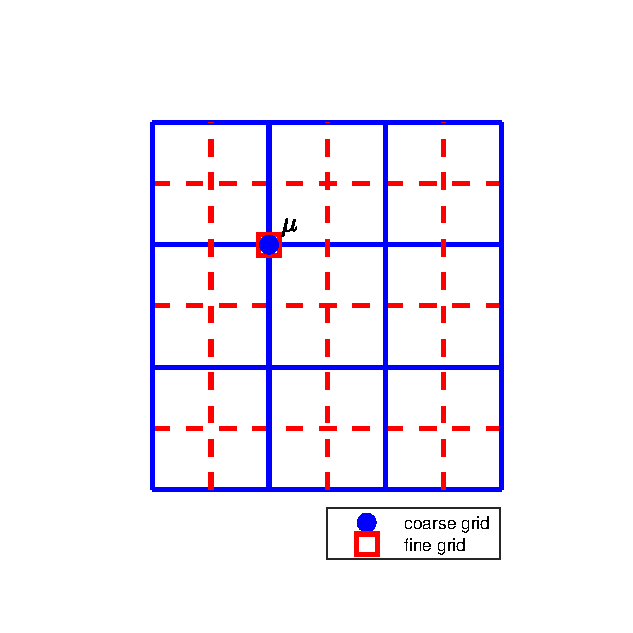
\includegraphics[width=0.24\textwidth,trim={1.8cm 0.8cm 1.4cm 1.2cm}, clip]{interpolation1.eps}
	\includegraphics[width=0.24\textwidth,trim={1.8cm 0.8cm 1.4cm 1.2cm}, clip]{interpolation2.eps}
	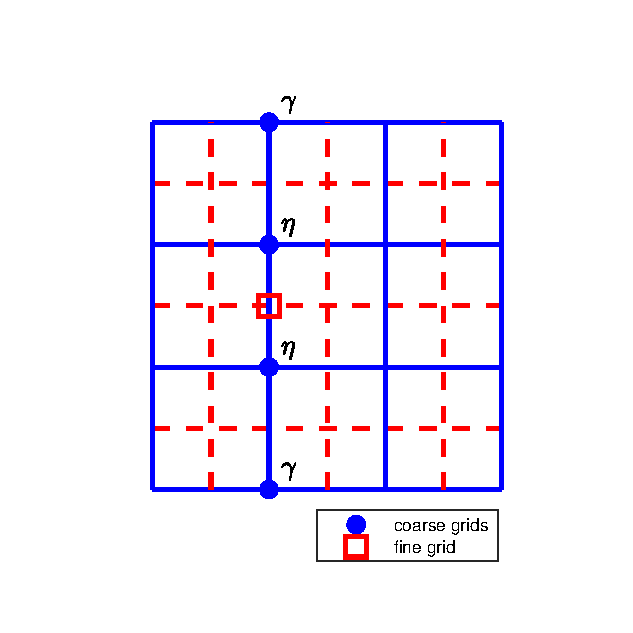
\includegraphics[width=0.24\textwidth,trim={1.8cm 0.8cm 1.4cm 1.2cm}, clip]{interpolation3.eps}
	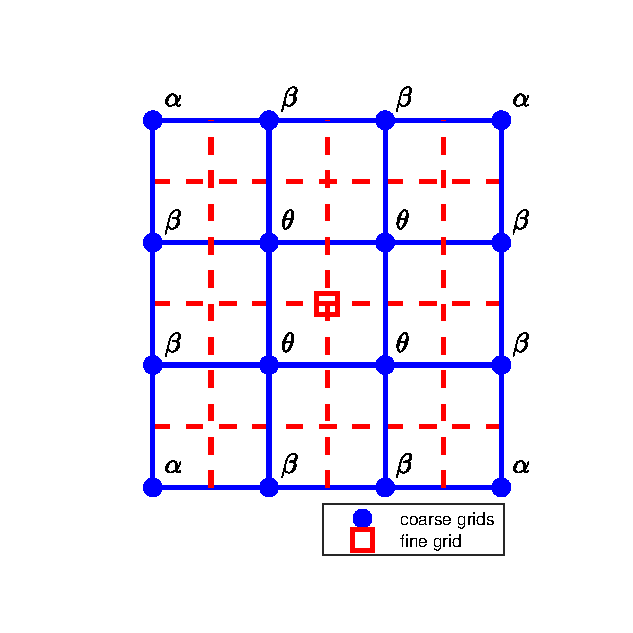
\includegraphics[width=0.24\textwidth,trim={1.8cm 0.8cm 1.4cm 1.2cm}, clip]{interpolation4.eps}
	\caption{The sketch for the stencils of fourth order interpolation operator ${\bf P}$ in two dimensions with parameters $\gamma = -\frac{1}{16}$, $\eta = \frac{9}{16}$, $\mu = 1$, $\alpha = \frac{1}{256}$, $\beta = -\frac{9}{256}$ and $\theta = \frac{81}{256}$. }\label{interpolation}
\end{figure}
\begin{figure}[htbp]
	\centering
	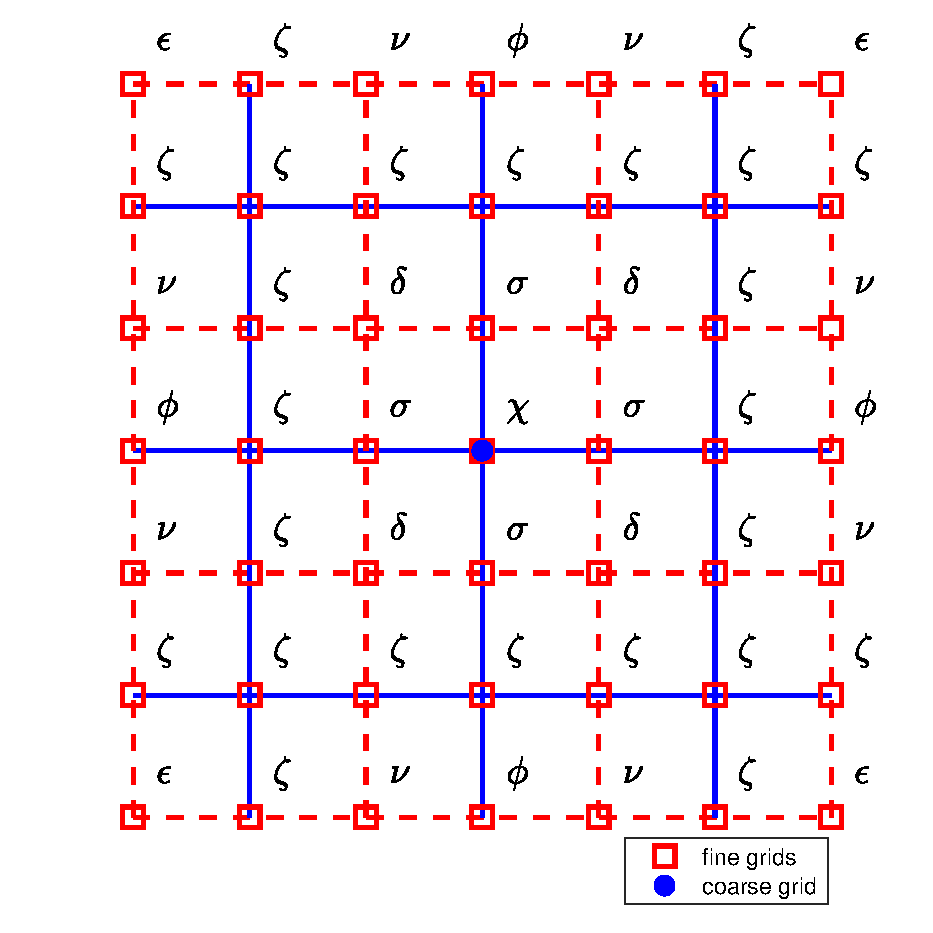
\includegraphics[width=0.6\textwidth]{restriction.eps}
	\caption{The sketch for the stencil of fourth order restriction operator ${\bf R}$ in two dimensions with parameters $\epsilon = \frac{1}{1024}$, $\nu = -\frac{9}{1024}$, $\phi = -\frac{16}{1024}$, $\delta = \frac{81}{1024}$, $\sigma = \frac{144}{1024}$, $\chi = \frac{256}{1024}$ and $\zeta = 0$.}\label{restriction}
\end{figure}




